
Traversal: Visiting all parts of the graph. Unlike linear data structures (Array, Linked List, Queues, Stacks, etc) which have only one logical way to traverse them, trees can be traversed in different ways. Following are the generally used ways for traversing trees.

\begin{figure}[H]
\centering
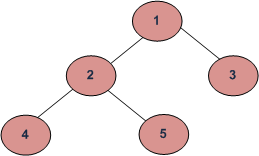
\includegraphics[width=0.3\textwidth]{tree12.png}
\end{figure}

\begin{itemize}
\item Depth First Traversals:
    \begin{itemize}
     \item Inorder (Left, Root, Right) : 4 2 5 1 3
     \item Preorder (Root, Left, Right) : 1 2 4 5 3
     \item Postorder (Left, Right, Root) : 4 5 2 3 1
    \end{itemize}
\item Breadth First or Level Order Traversal : 1 2 3 4 5

\end{itemize}

\subsection{Bread-first Search (BFS)}
Most of the cases, BFS is used to find out the shortest path from an unweighted 
and undirected graph.
\subsubsection{Basics}
\begin{itemize}
    \item Input:Graph $G = (V, E)$; a vertex $s$ as starting point.
    \item Goal: Visit all the vertices in systematic manner.
    \item Intuition: Think of the graph is drawn as a pond of water. Drop a 
stone at vertex v and watch the ripple expand with great regularity. The 
order of vertex visited in BFS is like the wave of ripples visiting the 
vertices.
\end{itemize}

\subsubsection{Algorithm}

\paragraph{3 possible states for each vertex:}
\begin{itemize}
 \item Undiscovered
 \item Discovered: Just find out this vertex and have not check its neighbors.
 \item Finished: discover the node and all its neighbors.
\end{itemize}
\paragraph{Queue:}
\begin{itemize}
 \item Initialized with just vertex $s$. $Q \leftarrow \{x\}$. x is discovered.
 \item Work the follows repeatedly:
 \begin{itemize}
  \item Pull a vertex out of the queue.
  \item Put all its neighbors into the queue as discovered.
 \end{itemize}
\end{itemize}

\paragraph{Example:}
An example of BFS starting from vertex $x$.
\begin{figure}[H]
\centering
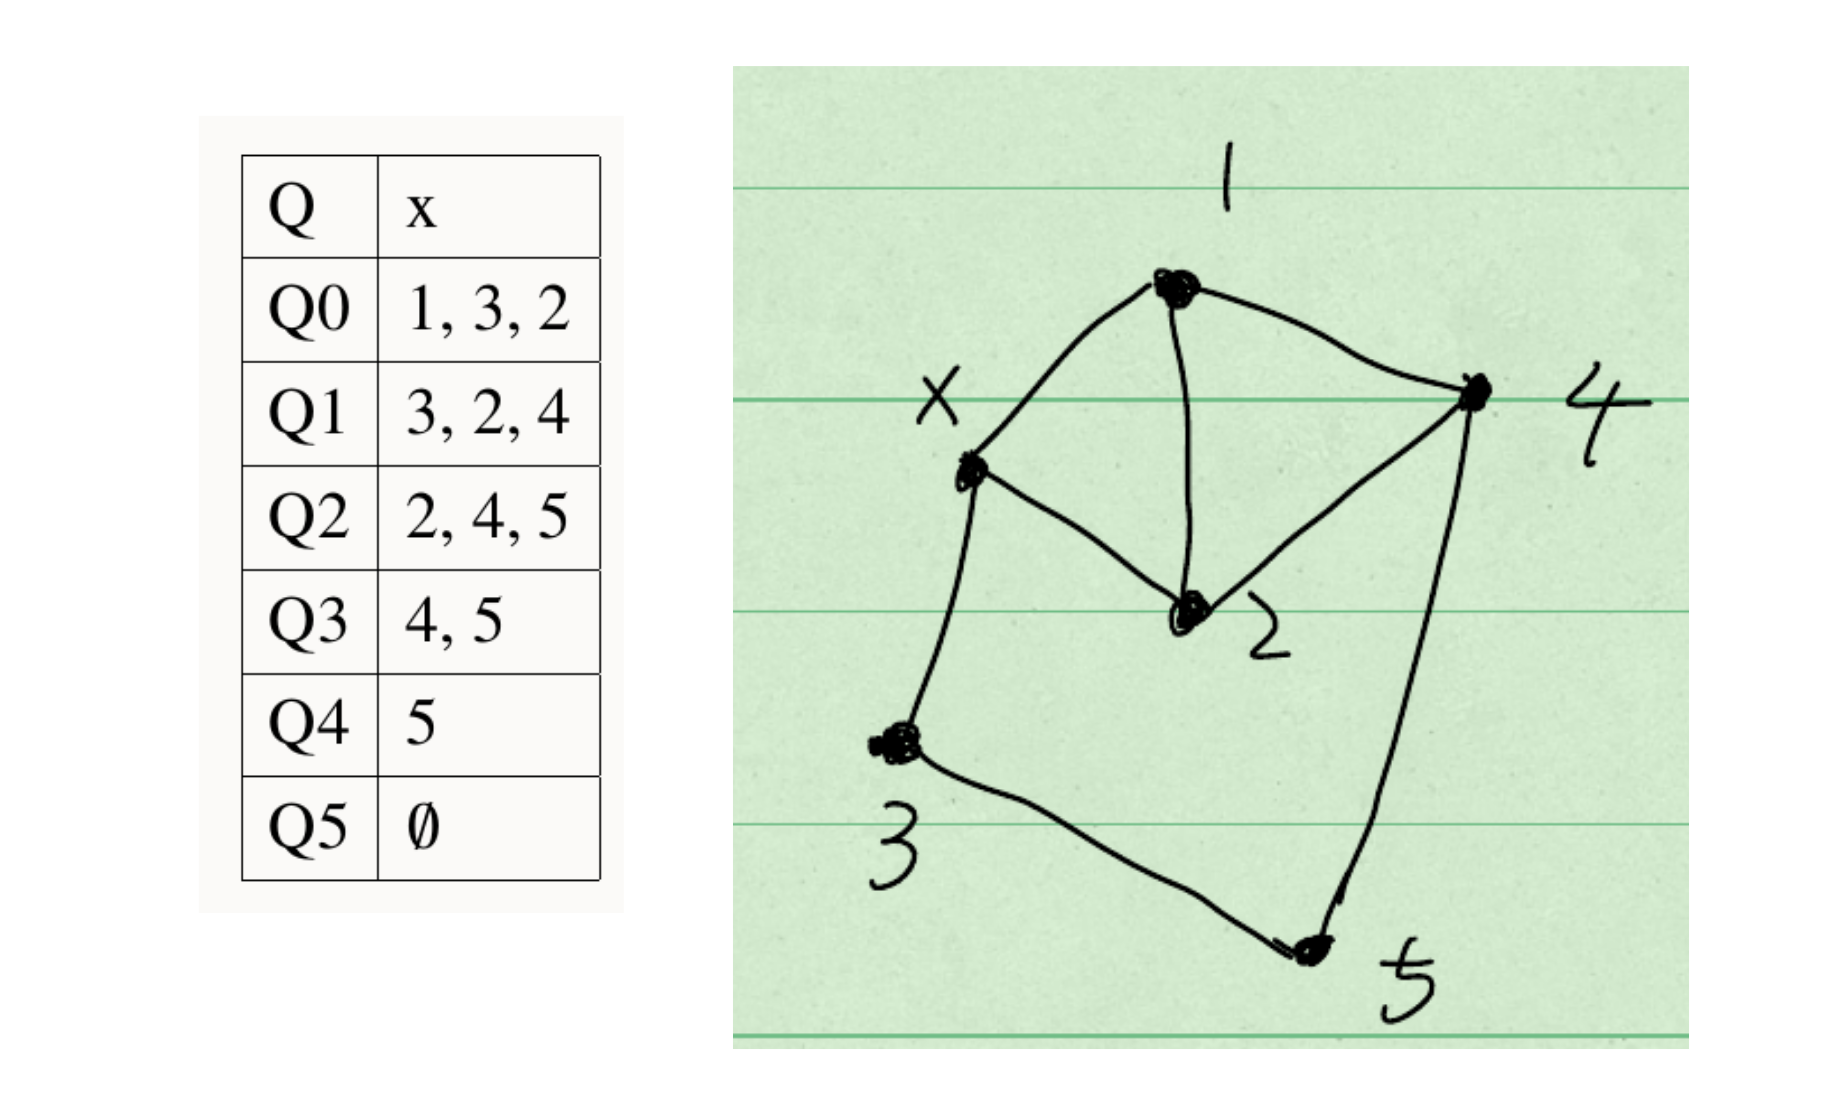
\includegraphics[width=0.5\textwidth]{queue.png}
\end{figure}

\paragraph{Remarks:}
\begin{itemize}
 \item In $Q1$, we did not put vertex $2$ into the queue since it is already in 
the Queue.
\item Vertices in queue are discovered.
\item Moving vertices out of the queue means it is finished.
\end{itemize}
\subsubsection{Levels}
\paragraph{Definition.}
Associate levels with vertices in BFS: 
\begin{itemize}
 \item The starting vertex is level 0: $\text{level}(s) = 0$.
 \item Any vertex $v$ is discovered when dequeue some vertex $u$, we set
\[\text{level}(v) = \text{level}(u) + 1\]
\end{itemize}

\begin{theorem}
 The level of $v$ is the smallest number of hops to get from $s$ to $v$.
\end{theorem}

\begin{proof}
 Let $\delta(s, v)$ be the smallest number of hops from $s$ to $v$. Prove that for any $v$, $\delta(s, v) = \text{level}(v)$.
\end{proof}

\begin{claim}
 $\delta(s, v) \le \text{level}(v)$.
\end{claim}

\begin{claimproof}
If $v$ has level $\text{level}(v)$, there is a sequence of vertices $$x, ~v_1, 
~v_2, ~\cdots, ~v_{\text{level}(v) - 1}, ~v$$, s.t. each one discovered from 
the previous.

We have shown one path from $x$ to $v$ which has $\text{level}(v)$ hops. 
Therefore, the smallest number of hops should be less or equal to the number of 
hops in this path. Therefore, $\delta(x, v) \le \text{level}(v)$.
\end{claimproof}
\begin{claim}
 $\delta(s, v) \ge \text{level}(v)$.
\end{claim}
\begin{claimproof}
Prove by contradiction. Suppose among all $v$ such that $\delta(s, v) < 
\text{level}(v)$, find the one with smallest $\delta(x, v)$.
\begin{figure}[H]
\centering
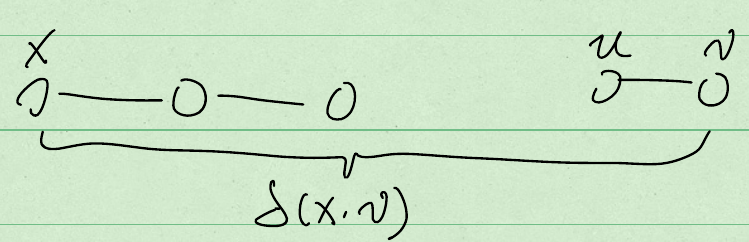
\includegraphics[width=0.5\textwidth]{level.png}
\end{figure}

Let $(s ~\cdots ~uv)$ be the path with fewest hops form $s$ to $v$.
\begin{align*}
&\delta(s, u) = \delta(s, v) - 1
\intertext{since $\delta(s, u) < \delta(s, v)$ and $\delta(s, v)$ is the 
smallest hops which less than level,}
\intertext{$\delta(s, u)$ must be larger than level$(u)$, i.e.}
&\text{level}(u) \le \delta(s, u) = \delta(s, v) - 1
\intertext{$v$ is the neighbor of $u$,}
&\text{level}(v) \le \text{level}(u) + 1 \le \delta(s, v)
\end{align*}
But we assume $\delta(s, v) < \text{level}(v)$, so we meet a contradiction the 
claim is true.
\paragraph{Notes}
\begin{itemize}
 \item $\text{level}(v) \le \text{level}(u) + 1$.\\
    Because $v$ can be discovered early than discovering from $u$.
\item Path $(s,v)$ is the shortest path which satisfies $\delta(s,v) < \text{level}(v)$. Therefore, any sub-path within $(s, v)$ has a $\delta$ greater than its level.
\end{itemize}
\end{claimproof}

\subsubsection{Remarks}
Look at edges on which new vertex are discovered. These edges from a tree and 
the discover sequence becomes the direction between vertices. Think 
of the tree are directed away from $s$, even though the graph is undirected.

Why it is a tree? Each vertex can be discovered at most one time. Every 
vertex at most have one in-coming edge then the graph is acyclic.

Will the tree contains all the vertices in the graph? 

No. The graph could have 
several isolated components. This is the expected result by design because BFS 
is used to find the shortest path from the source. So we do not want to find 
the vertex in different components because there is no path from the vertex to 
the source.

Will all the vertices in the same component with $s$ be discovered by BFS?
Prove by contradiction. There are some vertices in the component of $s$ that 
BFS starts which are not discovered. Among all such vertices, choose the one 
with the fewest hops away from the source.
% TODO: Prove it.
\subsection{Depth-first Search (DFS)}
The usage of DFS is broader than BFS. Explore one path as far as it will go, 
back track as little as needs. Repeat.

\subsubsection{Basics}

\paragraph{3 possible states for each vertex:}
\begin{itemize}
 \item Undiscovered
 \item Discovered: Just find out this vertex and have not check its neighbors.
 \item Finished: discover the node and all its neighbors.
\end{itemize}
\paragraph{Data Structure}
\begin{itemize}
\item BFS: Order of exploration of vertices is the same as the order of 
discovery. It is a FIFO, therefore we use queue to track discovered vertices.
\item DFS: Last discovered vertex is the first to be fully explored. It is a 
LIFO, therefore we use a stack to track the discovered vertices.
\end{itemize}
You get a stack for free by using recursion because during the recursion the 
OS maintains a stack by itself. Therefore, we can think about DFS as a 
recursive algorithm.

\subsubsection{Algorithm}
$DFS(G, s)$
\begin{itemize}
    \item Mark all vertices as undiscovered.
    \item Start with s and mark $s$ as discovered.
    \item While there is an undiscovered neighbor $u$ of $s$ call $DFS(G, u)$.
    \item Mark $s$ as finished.
\end{itemize}

\subsubsection{DFS Tree}
Formed by the set of edges on which new vertices are discovered. 

\begin{theorem}
In an undirected graph, if $(u, v)$ is an edge in the graph that is not in the DFS tree. Then $u$ is an ancestor of $v$ or $v$ is an ancestor of $u$ in the DFS tree.
\end{theorem}

\begin{proof}
% Should know the proof
Those edges are called ``back edges''. In an undirected graph you can only 
have tree edges and back edges.
\begin{figure}[H]
\centering
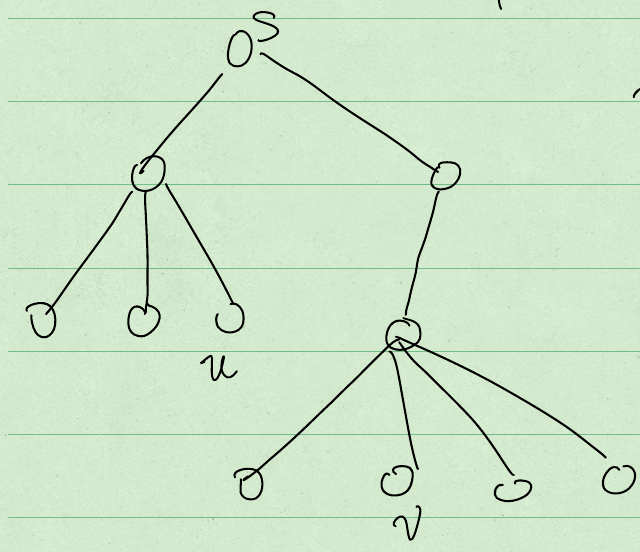
\includegraphics[width=0.5\textwidth]{dfs.png}
\end{figure}
This cannot exist because $v$ would have been discovered from $u$.
\end{proof}
\subsubsection{Time}
Suppose $u$ is a vertex in an undirected connected graph $G$.
\begin{itemize}
\item Time advance at each call and return of DFS function. The range of time 
is $[1, 2n]$.
\paragraph{Notes:} Every time you finish a recursive call of DFS, time advance 
by 1. Every time you make a new recursive call time advance by 1. Time is 
discrete and start from 1 at the first DFS call to $s$ and advance by 1 every 
time you finish or start a new recursive call.
\item $s(u)$: \textbf{The start time} of $u$ is the time at which DFS of $u$ is 
invoked.
\item $f(u)$: \textbf{The finish time} of $u$ is the time at which the DFS of 
$u$ is finished.
\end{itemize}
\subsubsection{Duration}
It is generally true for recursive function that the duration of an vertex $u$ 
is the integral from the start to the finish time.
\[\text{Duration}(u) = [s(u), f(u)]\]
$\forall u, v,$ it is not the case that 
\[s(u) < s(v) < f(u) < f(v)\]
Recursive algorithm ensures that it does not happen since it is last in first 
out. $v$ should finish first before $u$.

\subsubsection{Lineage}
\begin{itemize}
\item \textbf{Ancestor:} If you have a rooted tree, $u$ is call ancestor of 
$v$ if $u$ is on the path from $v$ to the root. 
\item \textbf{Descendant:} If $v$ is an ancestor of $u$, then $u$ is the 
descendant of $v$.
\item By convention, we include itself as ancestor so we allow $v$ to be its 
own ancestor as well as its own descendant.
\end{itemize}
\begin{theorem}
Suppose $u$ is discovered before $v$ and there is a path \textbf{of 
undiscovered vertices} between $u$ and $v$. Then $v$ will become a descendant 
of $u$.
\end{theorem}
\begin{proof}
Prove by contradiction. Suppose it is not the case and look at the first 
vertex on the path from u to v of undiscovered vertices that dose not become 
the descent of $u$.

Look at the first vertex to violate the rule would be a good way to prove a 
contradiction.
% TODO: prove this theorem
\end{proof}
\subsection{Notes}
BFS is used to find the shortest path from the source in the graph therefore we 
start BFS from the source until we exhaust the component where the source lies.

DFS is also used to get a global picture of the entire graph and we often want 
DFS to be deterministic enough. We start from the source and do DFS. We only 
discover the vertices in the connected component of that source. But we want to 
discover other vertices. So we have a outer layer to restart the DFS from some 
undiscovered vertices in some other component every time we finish the search 
within one component. In this way, DFS is able to cover all the vertices and 
all the components. Therefore, often you only need to give DFS a graph without 
any source explicitly.

Ideally, BFS and DFS are just different traversal strategies, so the total run time should be the same which is the number of nodes plus the number of edges. In practice, the running time depends on how to access the nodes and edges. By convention, assume $|V| = m$, $|E| = n$. If the graph is an adjacency matrix, the run time is $O(|m|^2)$. If the graph is an adjacency list, the run time is $O(|n| + |m|)$.